\documentclass[a4paper]{article} 

%中文环境设置
\usepackage{xeCJK} 
\usepackage{indentfirst}
\setlength{\parindent}{2em}
\usepackage{enumitem}

\usepackage{abstract}
\renewcommand{\abstractname}{摘要}
\providecommand{\keywords}[1]{\textbf{\textit{关键词}} #1}

\setCJKmainfont{STSong} % 中文主字体设置 

\usepackage[colorlinks,linkcolor=blue, citecolor=blue]{hyperref}

% 常用宏包
\usepackage{float}
\usepackage{stfloats}
\usepackage{graphicx}
\usepackage{color}

% 代码环境设置
\usepackage{listings}
\lstset{
	columns=fullflexible,
 	frame=single,
 	breaklines=true,
}
\definecolor{lightgray}{gray}{0.9}
\newcommand{\inlinecode}[2]{\colorbox{lightgray}{\lstinline[language=#1]$#2$}}

% 页面段落设置
\usepackage{multicol}
\usepackage{geometry}
\geometry{left=3.18cm, right=3.18cm, top=2.54cm, bottom=2.54cm}
\linespread{1.3}
%\setlength{\parskip}{0.5em} 

% 数学环境设置
\usepackage{amsmath}
\usepackage{amsthm}
\usepackage{amsfonts}
\newtheorem{myDef}{Definition} 
\newtheorem{myThm}{Theorem}
\newtheorem{myProp}{Property}

\begin{document} 
\title{线性方程组部分上机习题}
\author{吴佳龙 2018013418}
\date{}
\maketitle

\begin{abstract}
	通过理论分析和编程计算,运用不同算法分别求解系数矩阵为 Hilbert阵的病态线性方程组 $Hx=b$,比较他们的异同与优劣。运用的直接接法和迭代解法分别为:Gauss 消元法、Cholesky 分解方法、Tikhonov正则化改进的 Gauss 消元法和 Cholesky 方法;共轭梯度法和GMRES方法。
\end{abstract}

%\keywords{one, two, three, four}

\begin{multicols}{2}

\begin{section}{问题}

设 $H_{n}=\left[h_{i j}\right] \in \mathbb{R}^{n \times n}$ 是 Hilbert 矩阵,即 $$h_{i j}=\frac{1}{i+j-1}$$,取 $x=\left(\begin{array}{c}{1} \\ {\vdots} \\ {1}\end{array}\right) \in \mathbb{R}^{n}$,令 $b_n = H_nx$。再利用不同的数值方法求解病态线性方程组 $H_nx=b_n$。
	
\end{section}

\begin{section}{直接解法:Gauss 消元法和 Cholesky 分解方法}

	\begin{subsection}{列主元的 Gauss 消元法}
	
		\begin{subsubsection}{算法原理}
		
			对于线性方程组 $Ax=b$,若 $A$ 可逆且 $A$ 的顺序主子式都不为 $0$,则可将 $A$ 的每一列依次做初等变换 $L_n \cdots L_2 L_1A = \tilde{L}A = U$ 为上三角阵。由此可将 $Ax=b$ 转化为求解 $Ux = \tilde{L}b = \tilde{b}$ ,其中系数矩阵为上三角阵,可在 $O(n^2)$ 的复杂度内通过简单递推求得 $x$:
			
			$$x_i = (\tilde{b}_i - \sum_{j=i+1}^n U_{ij} x_{j}) / U_{ii}$$
			
			若 $A$ 的顺序主子式不全为 $0$,或者消元过程中主元 $|A_{ii}^{(i-1)}|$ 过小容易带来较大误差,可采用选取列主元的 Gauss 消元法。具体地,每次选取 
			
			$$pivot = \mathop{\arg\min}_{j\ge i} |A_{ji}^{(i-1)}|$$ 
			
			作为主元,交换行 $pivot$ 和行 $i$ 后再进行初等变换消元。该算法的矩阵表示为分解 $\tilde{L} P A = U$,将 $Ax=b$ 转化为求解 $Ux=\tilde{L}Pb$。
			
			Gauss消元法和选取列主元的Gauss消元法的总复杂度都为 $O(n^3)$
		
		\end{subsubsection}
	
		\begin{subsubsection}{误差分析}
		
			根据课本定理 4.4,可分析列主元的 Gauss 消元法的误差:
			
			\begin{myThm}
			
				设用列主元的Gauss消元法解 $Ax=b$,其计算解 $\tilde{x}$ 满足 $(A+\delta A)\tilde{x} = b$,并设 $nu\leq 0.01$,则有
				
				\begin{small}
				$$\frac{\|x-\tilde{x}\|_{\infty}}{\|x\|_{\infty}} \leq \frac{\operatorname{cond}(A)_{\infty}}{1-\left\|A^{-1}\right\|_{\infty}\|\delta A\|_{\infty}}\left[1.01\left(n^{3}+3 n^{2}\right) \rho u\right]$$
				\end{small}
			
			\end{myThm}
			
			定理中 $u$ 是机器精度,$\rho = \max_{1\leq i,j,k\leq n} |a^{(k)}_{ij}| / \|A\|_{\infty}$ 称为列主元 Gauss 消元法的增长因子。
			
			根据定理,计算解 $\tilde{x}$ 的相对误差受 $cond(A)$ 的影响很大。
			
		\end{subsubsection}
	
		\begin{subsubsection}{算法实现}
		
			列主元的 Gauss 消元法的 MATLAB 实现如下:
			
			\begin{lstlisting}[language=Matlab]
function [x] = myGauss(A, b)
% 选取列主元的高斯消元法 Ax=b
% 假定参数的size满足 A: [n,n], b: [n,1]
[n,~] = size(A);
A = [A, b]; % 增广矩阵
% 选取列主元的高斯消元
for i = 1:n
    [~, pivot] = max(abs(A(i:end, i)));
    pivot = pivot + i - 1; % 列主元
    A([i,pivot],:) = A([pivot,i],:);
    scale = A(i+1:end, i) / A(i,i);
    A(i+1:end, :) = A(i+1:end, :) - scale * A(i, :);    
end
% 解 Ux=b1
x = zeros(n,1);
x(n) = A(n,end) / A(n,n);
for i = n-1:-1:1
    x(i) = (A(i, end) - A(i, i+1:end-1) * x(i+1:end)) / A(i,i);
end
end

			\end{lstlisting}
		
		\end{subsubsection}
	
	\end{subsection}
	
	\begin{subsection}{Cholesky 分解方法}
	
		\begin{subsubsection}{算法原理}
		
			对于系数矩阵对称正定的方程组 $Ax=b$,可将系数矩阵分解为下三角及其转置的乘积:
			
			$$A = LL^T$$
			
			根据系数关系可得 $L$ 各元素的计算公式:
			
			$$l_{jj} = (a_{jj}-\sum_{k=1}^{j-1}l_{jk}^2)^{1\over 2}$$
			$$l_{ij} = {1\over l_{jj}} (a_{ij} - \sum_{k=1}^{j-1}l_{ik}l_{jk}), i=j+1,\cdots,n$$
			
			该分解将 $Ax=b$ 转化为求解 $Ly=b$ 和 $L^Tx=y$ 两个方程组,他们的系数矩阵分别为下三角和上三角。
			
			该算法的复杂度为 $O(n^3)$。相比 Gauss 消元法,该算法的时间和空间复杂度的常数较小。
		
		\end{subsubsection}
	
		\begin{subsubsection}{误差分析}
		
			该分解方法是 Gauss 消元法的变形,其误差也直接受到系数矩阵条件数 $cond(A)$ 的影响。
			
		\end{subsubsection}
	
		\begin{subsubsection}{算法实现}
		
			Cholesky 分解方法求解线性方程组的 MATLAB 实现如下:
			
			\begin{lstlisting}[language=Matlab]
function [x] = myCholesky(A, b)
% cholesky分解方法求解 Ax=LL'x=b
% 假定参数的size满足 A: [n,n], b: [n,1]
[n,~] = size(A);
% Cholesky 分解
L = zeros(n,n);
for j = 1:n
    L(j,j) = sqrt(A(j,j) - sum(L(j, 1:j-1).^2));
    L(j+1:n, j) = ( A(j+1:n,j) -  L(j+1:n,1:j-1)*L(j,1:j-1)') / L(j,j); 
end
% Ly=b
y = zeros(n,1);
y(1) = b(1) / L(1,1);
for i = 2:n
    y(i) = (b(i) - L(i,1:i-1)*y(1:i-1)) / L(i,i);
end
% L'x=y
x = zeros(n,1);
L_t = L';
x(n) = y(n) / L_t(n,n);
for i = n-1:-1:1
    x(i) = (y(i) - L_t(i, i+1:end) * x(i+1:end)) / L_t(i,i);
end
end
			\end{lstlisting}
		
		\end{subsubsection}
		
	\end{subsection}
	
\end{section}

\begin{section}{Tikhonov 正则化方法改进系数矩阵条件数}

	\begin{subsection}{算法原理}
	
		对于病态的方程组,做某些预处理,可以降低系数矩阵的条件数,其中最有效的是 Tikhonov 正则化方法。
		
		该方法将 $Ax=b$ 转化为求解 
		
		$$(\alpha I+A^HA)x_{\alpha} = A^Hb$$
		
		该方程可用直接解法(Gauss 消元法等)求解,但是其系数矩阵的行列式 $$cond_2(\alpha I+A^HA) = {\frac{\alpha+\mu_{1}^{2}}{\alpha+\mu_{n}^{2}}}$$ 当 $\alpha > \mu_1\mu_n$ 时小于原矩阵条件数 $\mu_1\over\mu_n$。
		
		又,
		\begin{align*}
		  \left\|\mathbf{x}_{\alpha}-\mathbf{x}\right\|_{2} &\leq\left\|\left(\alpha I+A^{H} A\right)^{-1} A^{H}\right\|_{2} \cdot \delta \\
		  &+\left\|\left(\alpha I+A^{H} A\right)^{-1} A^{H} \mathbf{b}-A^{+} \mathbf{b}\right\|_{2}
		\end{align*}
			
		其中 $\delta$ 表示 $b$ 的扰动带来的误差。若让上式右端两项量级大致相同,可取
		
		$$\mu_{1} \mu_{n}<\alpha \sim \mathcal{O}\left(\mu_{1}^{2} \delta\right)$$
		
	\end{subsection}
	
	\begin{subsubsection}{算法实现}
	
		Tikhonov 正则化方法的 MATLAB 实现如下:
		
		\begin{lstlisting}[language=Matlab]
function [x] = myTikhonov(A, b, delta, directMethod)
% Tikhonov正则化方法改进条件数求解 Ax=b
% 假定参数的size满足 A: [n,n], b: [n,1]
% directMethod为直接解法的函数指针
%  如 @myGauss @myCholesky
[n,~] = size(A);
eigen = eig(A);
miu1 = eigen(end);
alpha = miu1^2*delta;
% 调用直接解法求解改进后的方程组
x = directMethod(alpha*eye(n)+A'*A, A'*b);
end

		\end{lstlisting}
	
	\end{subsubsection}

\end{section}

\begin{section}{迭代解法:共轭梯度法和 GMRES 方法}

	\begin{subsection}{共轭梯度法及预处理共轭梯度法}
	
		\begin{subsubsection}{算法原理}
		
			对于对称正定阵 $A$,方程组 $Ax^{*}=b$ 等价于变分问题 
			
			$$\varphi(x^*) = \min_{x\in \mathbb{R}^n} \varphi(x)$$
			
			我们可以用最速下降法求解该最小化问题,但是当 $A$ 的条件数很大时,最速下降法收敛很慢。
			
			我们可以构造一组 $A$-共轭向量组 $\{p^{(i)}\}$,满足 $(Ap^{(i)},p^{(j)})=0, i\ne j$,且具有较好的性质:依次对 $p^{(1)},\cdots,p^{(l)}$ 进行一维极小搜索后的结果就是在 $\text{span}\{p^{(1)},\cdots,p^{(l)}\}$ 上的最小值。该算法称为共轭梯度法(CG算法)。
			
			课本95页给出CG算法产生的序列有如下性质:
			
			\begin{myProp}
				$A$ 对称正定,记 $K = cond_2(A)$,则
				$$\left\|\mathbf{x}^{(k)}-\mathbf{x}^{*}\right\|_{A} \leq 2\left(\frac{\sqrt{K}-1}{\sqrt{K}+1}\right)^{k}\left\|\mathbf{x}^{(0)}-\mathbf{x}^{*}\right\|_{A}$$
			\end{myProp}
			
			可见当 $A$ 病态时,CG算法仍然收敛很慢,预先设法降低条件数,就是预处理的共轭梯度法(PCG算法)。
			
			PCG算法选取一个对称正定阵 $M=SS^T$,将 $Ax=b$ 改写为等价方程组:
			
			$$S^{-1}AS^{-T}u = S^{-1}b,\ x=S^{-T}u$$
			
			然后用CG法求解第一个方程。这样,在解的迭代序列仍满足上述性质中,不过其中 $K=cond(M^{-1}A)_2$。
			
			$M$ 的常见选取有:$A$ 的不完全Cholesky分解、Jacobi迭代法的分裂矩阵 $M=D$、SSOR法的分裂矩阵等。
		
		\end{subsubsection}
	
		\begin{subsubsection}{算法描述}
		
			CG算法的描述如下:
			
			\begin{enumerate}
			  \item 任取 $x^{(0)} \in \mathbb{R}^{n}$
			  \item $r^{(0)}=b-A x^{(0)}, p^{(0)}=r^{(0)}$
			  \item 对 $k=0,1,\cdots,$ $$\begin{array}{l}{\alpha_{k}=\frac{\left({r}^{(k)}, {r}^{(k)}\right)}{\left({p}^{(k)}, {A} {p}^{(k)}\right)}} \\ {{x}^{(k+1)}={x}^{(k)}+{\alpha}_{k} {p}^{(k)}} \\ {{r}^{(k+1)}={r}^{(k)}-{\alpha}_{k} {A} {p}^{(k)}} \\ {{\beta}_{k}=\frac{\left({r}^{(k+1)}, {r}^{(k+1)}\right)}{\left({r}^{(k)}, {r}^{(k)}\right)}} \\ {{p}^{(k+1)}={r}^{(k+1)}+{\beta}_{k} {p}^{(k)}}\end{array}$$
			\end{enumerate}
			
			PCG算法的描述如下:
			
			\begin{enumerate}
			  \item 任取 $x^{(0)} \in \mathbb{R}^{n}$
			  \item $r^{(0)}=b-A x^{(0)}, z^{(0)}=M^{-1} r^{(0)}, p^{(0)}=z^{(0)}$
			  \item 对 $k=0,1,\cdots,$ $$\begin{array}{l}{\alpha_{k}=\frac{\left(z^{(k)}, r^{(k)}\right)}{\left(p^{(k)}, A p^{(k)}\right)}} \\ {x^{(k+1)}=x^{(k)}+\alpha_{k} p^{(k)}} \\ {r^{(k+1)}=r^{(k)}-\alpha_{k} A p^{(k)}} \\ {M z^{(k+1)}=r^{(k+1)}}  \\ {\beta_{k}=\frac{\left(z^{(k+1)}, r^{(k+1)}\right)}{\left(z^{(k)}, r^{(k)}\right)}} \\ {p^{(k+1)}=z^{(k+1)}+\beta_{k} p^{(k)}}\end{array}$$
			\end{enumerate}
			
		\end{subsubsection}
	
		\begin{subsubsection}{算法实现}
			共轭梯度法(CG算法)的 MATLAB 实现如下:
			
			\begin{lstlisting}[language=Matlab]
function [x, iters] = myCG(A, b, kmax, eps)
% 共轭梯度法 Ax=b
% 假定参数的size满足 A: [n,n], b: [n,1]
% 返回值 iter 表示收敛时迭代次数
[n,~] = size(A);
x = zeros(n,1);
r = b-A*x;  p = r;
for k = 1:kmax
    alpha = (r'*r)/(p'*(A*p));
    x = x+alpha*p;
    last_r = r; r = r-alpha*A*p;
    beta = (r'*r)/(last_r'*last_r);
    p = r*beta+p;
    if norm(r)/norm(b) < eps
        iters = k;
        return;
    end
end
iters = kmax;
end
			\end{lstlisting}
			
			预处理共轭梯度法(PCG算法)的 MATLAB 实现如下:
			
			\begin{lstlisting}[language=Matlab]
function [x, iters] = myPCG(A, b, kmax, eps)
% 预处理的共轭梯度法 Ax=b
% 假定参数的size满足 A: [n,n], b: [n,1]
% 返回值 iter 表示收敛时迭代次数
[n,~] = size(A);
M = diag(diag(A)); % Jacobi迭代的分裂矩阵
x = zeros(n,1);
r = b-A*x; z = M\r; p = z;
for k = 1:kmax
    alpha = (z'*r)/(p'*(A*p));
    x = x+alpha*p;
    last_r = r; r = r-alpha*A*p;
    last_z = z; z = M\r;
    beta = (z'*r)/(last_z'*last_r);
    p = z+beta*p;
    
    if norm(r)/norm(b) < eps
        iters = k;
        return;
    end
end
iters = kmax;
end
			\end{lstlisting}
		
		\end{subsubsection}
		
	\end{subsection}
	
	\begin{subsection}{GMRES 方法}
	
		\begin{subsubsection}{算法原理}
		
			关于线性方程组,有Galerkin原理:$K_m$ 和 $L_m$ 是 $\mathbb{R}^n$ 中的两个 $m$ 维子空间,他们的基分别为 $\{v_i\}, \{w_i\}$,并记 $V_m = (v_1,\cdots,v_m), W_m = {w_1,\cdots,w_m}$。对于方程组 $Az=r_0$,在子空间 $K_m$ 中可以找到近似解$z_m$ 使得 $r_0-Az_m \perp L_m$。将 $z_m$ 表示为 $z_m = V_m y_m$,若 $W_m^TAVm$ 非奇异,解得
			$$z_m = V_m(W_m^TAV_m)^{-1}W_m^Tr0$$
			
			在 GMRES 算法中,取 $K_m = \text{span}\{r_0,\cdots, A^{m-1}r_0\}$,$ L_m=AK_m=\{Ar_0, \cdots, A^mr_0\}$,可以证明此时 $W_m^TAV_m$ 非奇异,且求解 $z_m$ 等价于在 $K_m$ 中极小化 $R(x)=\|\mathbf{b}-A \mathbf{x}\|_{2}^2$,即 $$R(\mathbf{x}_{0}+z_m)=\min _{\mathbf{x} \in \mathbf{x}_{0}+K_{m}} R(\mathbf{x})$$
			
			另外,可以证明,取 $\mathbf{v}_{1}=\mathbf{r}_{0} /\left\|\mathbf{r}_{0}\right\|_{2}$ 通过 Arnoldi 过程,可以将 $A$ 分解为 $$AV = VH$$,其中 $H$ 是上Hessenberg阵,$V = (v_1, \cdots, v_n)$ 是正交阵,且 $V_m = (v_1,\cdots,v_m)$ 是 $K_m$ 的一组标准正交基。
			
			有了上述 $A$ 的分解式,可以证明极小化残差 $R(x_0+z_m) = \|r_0-Az_m\|^2$ 等价于极小化 $\| \beta \mathbf{e}_{1}-\widetilde{H}_{m} \mathbf{y}_{m}\|$,其中 $\beta = \|r_0\|$, $\tilde{H}_{m}=\left(\begin{array}{c}{H_{m}} \\ {h_{m+1, m} \mathbf{e}_{m}^{T}}\end{array}\right)$。
		
		\end{subsubsection}
		
		\begin{subsubsection}{算法描述}
		
			GMRES算法描述如下:
			
			\begin{enumerate}
			  \item 选取适当的 $m, \mathbf{x}_0$,记 $\mathbf{r}_0 = \mathbf{b}-A\mathbf{x}_0, \beta = \|\mathbf{r}_0\|, \mathbf{v}_1 = \mathbf{r}_0/\beta$
			  \item 用Arnoldi过程求出 $V_m$ 和 $\widetilde{H}_{m}$
			  \item 求解最小二乘问题 $$\min _{\mathbf{y}_{m} \in \mathbb{R}^{m}}\left\|\beta \mathbf{e}_{1}-\widetilde{H}_{m} \mathbf{y}_{m}\right\|$$ 得到 $y_m$
			  \item 计算 $\mathbf{x}_{m}=\mathbf{x}_{0}+V_{m} \mathbf{y}_{m}, \mathbf{r}_{m}=\mathbf{b}-A \mathbf{x}_{m}$
			  \item 若 $\left\|\mathbf{r}_{m}\right\|<\varepsilon$ 则停止迭代,否则 $\mathbf{x}_{0}=\mathbf{x}_{m}, \mathbf{r}_{0}=\mathbf{r}_{m}, \mathbf{v}_{1}=\mathbf{r}_{m} /\left\|\mathbf{r}_{m}\right\|$,转第 2 步
			\end{enumerate}
		
		\end{subsubsection}
	
		\begin{subsubsection}{算法实现}
		
			GMRES算法的 MATLAB 实现如下:
			
			\begin{lstlisting}[language=Matlab]
function [x, iters] = myGMRESm(A, b, m, kmax, eps)
% GMRES算法求解 Ax=b
% 假定参数的size满足 A: [n,n], b: [n,1]
[n,~] = size(A);
m = min(m,n);
x0 = zeros(n,1);
% x0 = randn(n,1)*0.0001;
for k = 1:kmax
    r0 = b-A*x0;
    v1 = r0/norm(r0);
    % Arnoldi过程
    Vm = zeros(n,m+1); Vm(:,1) = v1;
    Hm = zeros(m+1,m);
    success = true;
    for i = 1:m
        for j = 1:i
            Hm(j,i) = dot(A*Vm(:,i), Vm(:,j)) / dot(Vm(:,j),Vm(:,j));
        end
        ri = A*Vm(:,i) - Vm(:,1:i)*Hm(1:i,i);
        if ~any(ri(:)) 
            success = false;
            break
        end % ri==0,中断
        if i<n
            Hm(i+1,i) = norm(ri);
            Vm(:,i+1) = ri/norm(ri);
        end
    end
    if ~success 
        x0 = randn(n,1)*0.0001;
        continue
    end % 若Arnoldi过程中断,重新选取x0
    Vm = Vm(:,1:m);
    % Arnoldi过程结束
    ym = Hm\(norm(r0)*speye(m+1,1));
    xm = x0+Vm*ym;
    rm = b-A*xm;    
    if norm(rm)/norm(b)<eps
        x = xm;
        iters = k;
        return
    else
        x0 = xm;
    end
end
iters = kmax;
x = xm;
end
			\end{lstlisting}
		
		\end{subsubsection}
	
	\end{subsection}
	
\end{section}

\begin{section}{计算结果与方法比较}

	\begin{subsection}{比较相对误差}
		对于 $n=2,3,\cdots,20$,分别计算 Gauss 法、Cholesky 法、 Tikhonov改进的 Gauss 法、Tikhonov改进的 Cholesky 法、PCG法、GMRES法的相对误差。其中 Tikhonov 正则化的参数设定为 $\delta = 10^{-13}$,PCG 参数指定为 $\varepsilon = 10^{-15}, kmax = 10000$,GMRES参数指定为 $m=5, \varepsilon = 10^{-15}, kmax = 10000$。如图 \ref{re} 所示:
		
		\begin{figure*}[ht] %h默认参数是可以浮动,不是固定在当前位置。如果要不浮动,你就可以使用大写float宏包的H参数,固定图片在当前位置,禁止浮动。
			\centering %使图片居中显示
			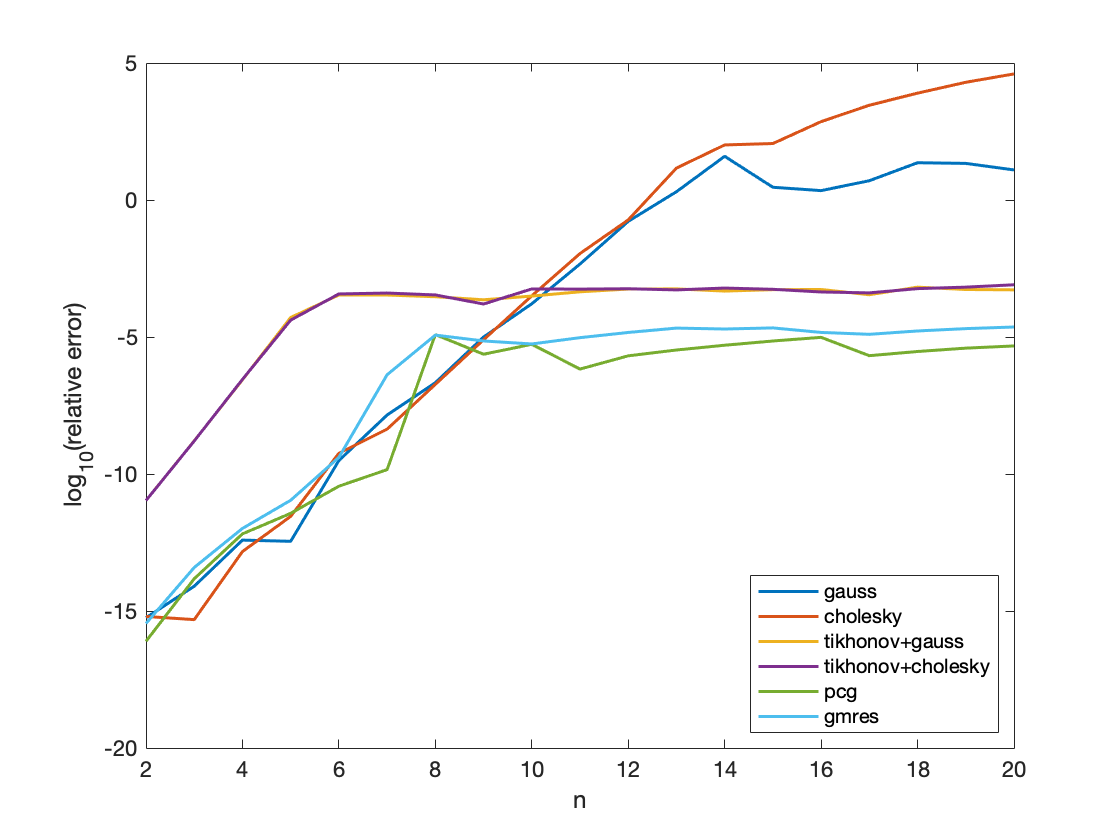
\includegraphics[width = \textwidth]{img/relative_error.png} 
			\caption{不同算法的相对误差}
			\label{re} 
		\end{figure*}
		
		另外对于 $n=100$,计算上述算法的相对误差:
		
		\begin{table}[H]
		\centering
		\begin{tabular}{|l|l|}
		\hline
		算法                & 相对误差       \\ \hline
		Gauss             & 3.6024e+03 \\ \hline
		Cholesky          & 7.3455e+18 \\ \hline
		Tikhonov+Gauss    & 5.7705e-04 \\ \hline
		Tikhonov+Cholesky & 7.8701e-04 \\ \hline
		PCG               & 6.2216e-06 \\ \hline
		GMRES             & 9.2631e-05 \\ \hline
		\end{tabular}
		\end{table}
		
		可以看到,随着 $n$ 的不断增大,Gauss 和 Cholesky 法的相对误差增长极其迅速,这是由于 $H$ 的条件数增长造成的,而采用 Tikhonov 正则化方法改进的直接解法以及迭代解法 PCG 和 GMRES 则都能保持相对误差的稳定。在文中实现的这些算法而言,迭代解法的相对误差较优于正则化后的直接解法。

	\end{subsection}
	
	\begin{subsection}{GMRES中m的选择}
		对于 $m=2,\cdots, n$,分别计算GMRES需要迭代的次数,此处设定参数 $\varepsilon = 10^{-8}, kmax=10000$。
		
		选取 $n=20$, 如图所示:
		
		\begin{figure}[H]
			\centering
			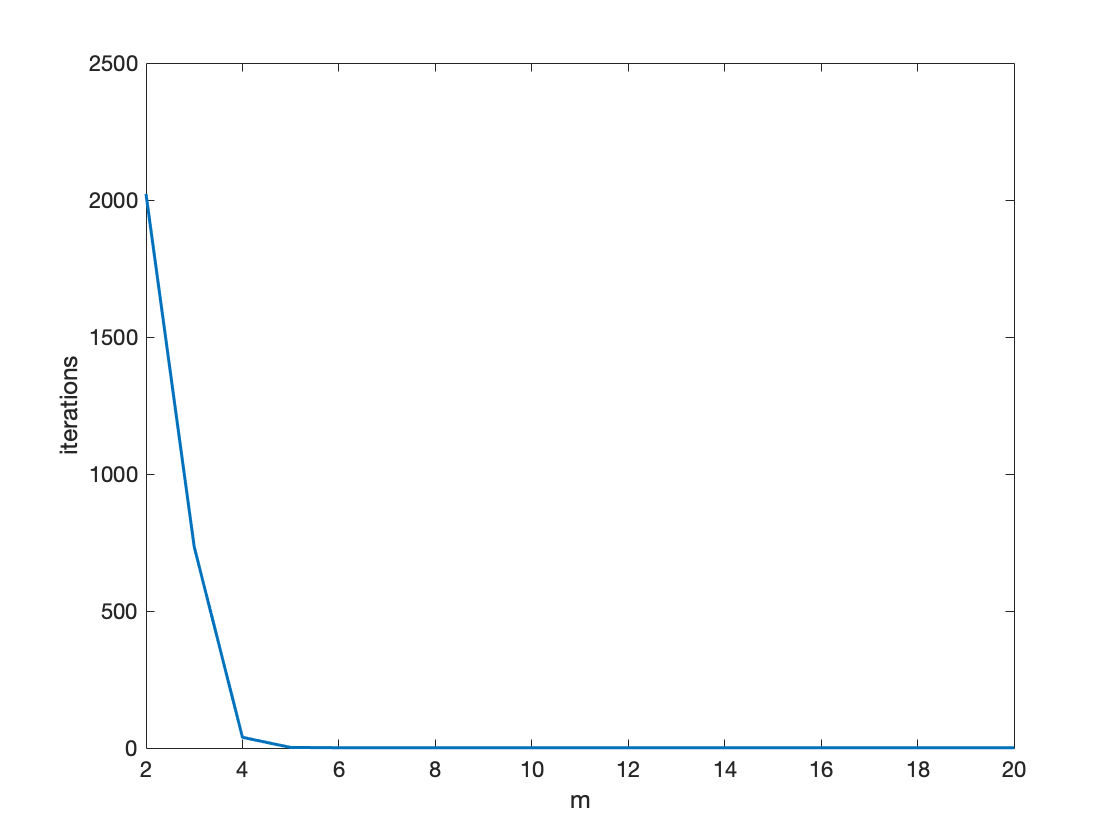
\includegraphics[width = 0.55\textwidth]{img/gmres20.png} 
			\label{gmres20} 
		\end{figure}
		
		选取 $n=200$,如图所示:
		
		\begin{figure}[H]
			\centering
			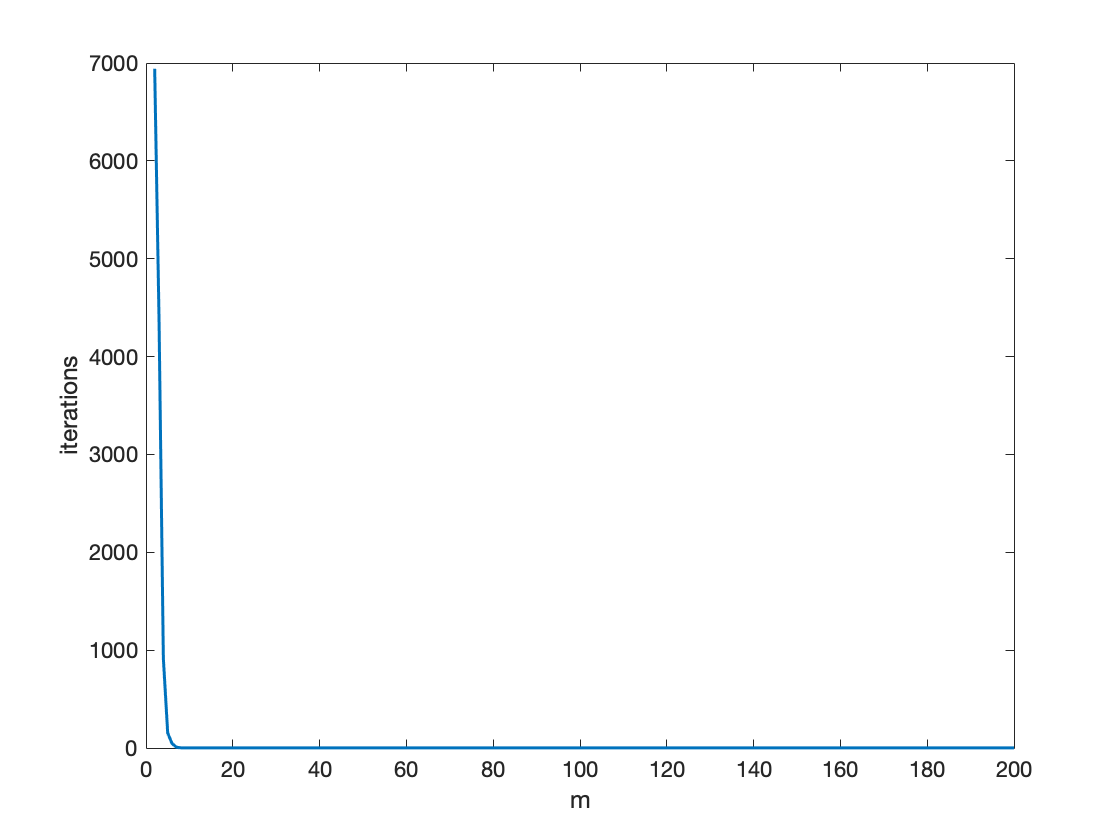
\includegraphics[width = 0.55\textwidth]{img/gmres200.png} 
			\label{gmres200} 
		\end{figure}
		
		可以看到,GMRES 收敛的迭代次数随着 m 的增加迅速下降,这为以下两个实验以及解方程组的实际运用提供了选择合适的 $m$ 的经验。
	\end{subsection}

	\begin{subsection}{比较迭代次数}
		比较 CG、PCG、GMRES的迭代次数,设定参数 $\varepsilon = 10^{-8}, kmax=10000$, GMRES分别设置参数 $m=2,5,10$。如图所示:
		
		\begin{figure}[H]
			\centering
			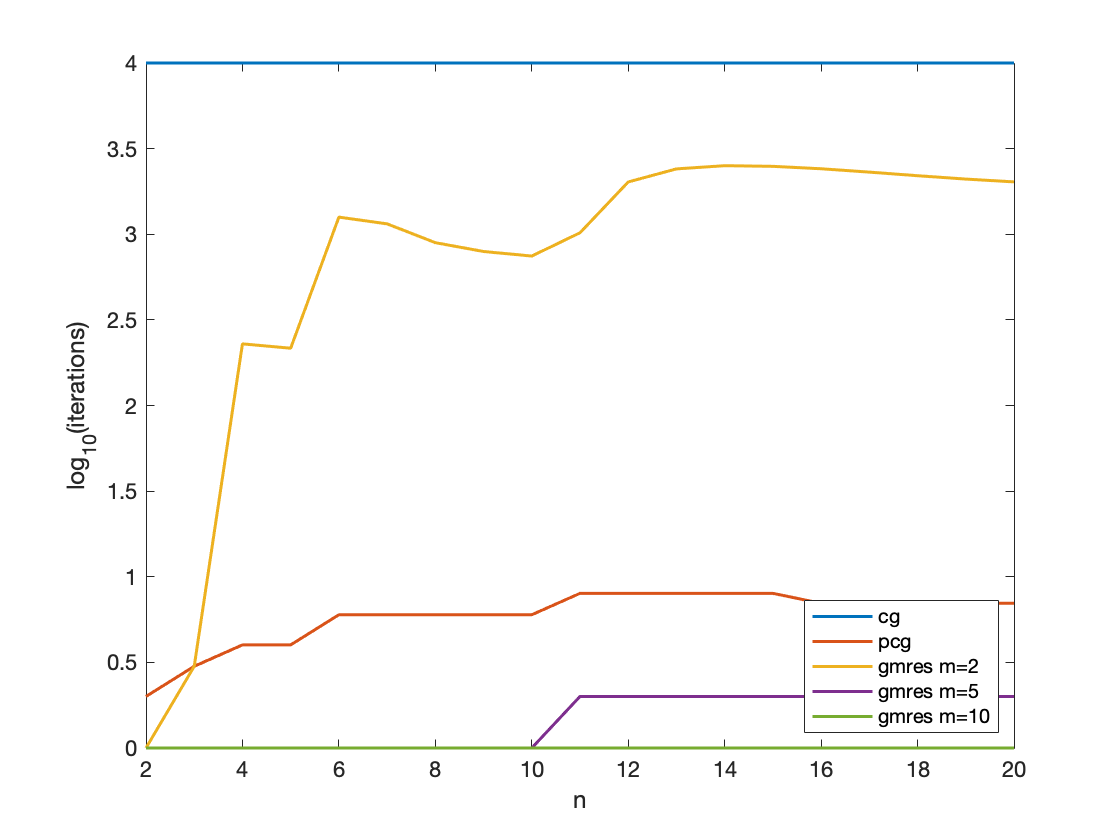
\includegraphics[width = 0.55\textwidth]{img/iterations.png} 
			\label{iter} 
		\end{figure}
		
		对于病态的系数矩阵 $H$,CG算法的收敛速度显著慢于其他算法。对于 PCG 和 GMRES 算法的比较,参数 $m$ 的选择较为重要。
	\end{subsection}
	
	\begin{subsection}{比较迭代时间}
		比较 PCG 和 GMRES 的计算时间,设定参数 $\varepsilon = 10^{-8}, kmax=10000$, GMRES分别设置参数 $m=\max(\lfloor n/10 \rfloor, 10)$。运行时间随着计算机状态变化而不稳定,其中一次运行结果如图所示:
		
		\begin{figure}[H]
			\centering
			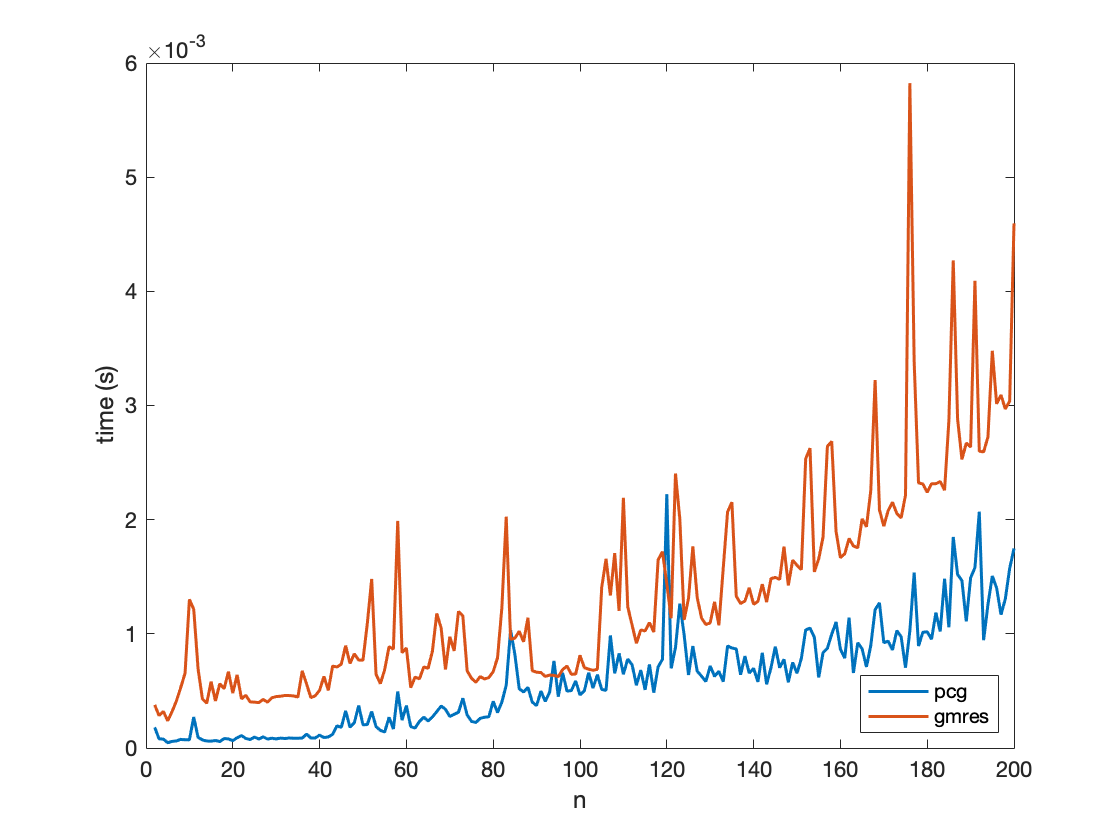
\includegraphics[width = 0.55\textwidth]{img/time.png} 
			\label{time} 
		\end{figure}
		
		进行多次运行后总结规律发现,在文中对于 PCG 和 GMRES 的这种具体实现下,当 $n$ 较大时,PCG 比 GMRES 的收敛速率稍快些。另外,GMRES 的运行时间不仅取决于收敛速率还取决于一次迭代所需的时间,这里所取的 $m=\max(\lfloor n/10 \rfloor, 10)$ 只是凭直觉选择,并不是理论上使算法最快的 $m$。PCG 与 GMRES 的效率比较要综合考虑各方面的因素。
	\end{subsection}

\end{section}

\begin{section}{总结}
	本次实验对于几种不同的解线性方程组的算法进行了理论分析和编程计算,这些算法分别是:Gauss 消元法、 Cholesky 分解⽅法、Tikhonov 正则化改进的 Gauss 消元法和 Cholesky ⽅法;共轭梯度法和 GMRES ⽅法。通过求解具体的病态线性方程组 $Hx = b$,显示了未经正则化的直接解法的结果具有极大的误差,而正则化后的直接解法以及迭代解法的相对误差能稳定在较小的范围。
	另外,还对迭代解法的收敛速率和运行时间运行了实验进行探索,并未得出显著的结论,实际上,方法本无绝对的优劣。
\end{section}

\end{multicols}



%\bibliographystyle{unsrt}
%\bibliography{ref.bib}

%\begin{thebibliography}{99}    %参考文献开始
%	\bibitem{ml}周志华. 机器学习[M]. 清华大学出版社, 2016.   
%\end{thebibliography}	

\end{document}

